Le but de cette section est d'analsyer quels sont les besions des différents utilisateurs et de trouver quelle est la meilleure manière d'y répondre. Un autre point très important est le détails des choix technologiques. Je vais donc tous les passer en revue et les expliquer.
\section{Besoins}

Dans un premier temps, il convient d'identifier quels seront les différents types d'utilisateurs de cette plateforme de quiz. Il y a selon moi deux types bien distinct d'utilisateurs :
\begin{itemize}
    \item Les étudiants
    \item Les professeurs
\end{itemize}

Les premiers utilisent cette plateforme afin de répondre à des quizs. La forme de ces derniers peuvent varier entre un simple quiz pour valider un devoir, un drill dans le but de réviser un examen ou finalement l'examen en lui-même. Ils ont donc besoin d'une interface où ils peuvent voir et choisir un quiz parmi tous ceux dont l'accès leurs est autorisé. Il doit pouvoir répondre au quiz et dans le cadre d'un examen ou d'un devoir il doit pouvoir le rendre. Il doit également pouvoir naviguer dans le quiz.

Les professeurs quant à eux ont des besoins bien différents. Ils veulent principalement créer des quizs avec des questions de plusieurs types tels que un QCM, des textes à trous ou encore des questions de code. Ils doivent également pouvoir regrouper leurs étudiants en différentes classes et autoriser cette classe à répondre à certains quizs. Dernièrement, ils ont besoin de pouvoir corriger automatiquement certaines questions comme les QCM.

%TODO : Mettre digramme



\section{Technologies}
\subsection{Technologies présentes dans l'application}
Je vais brièvement rappeler les choix technologiques qui ont déjà été pris pour ce projet :
\begin{itemize}
    \item Pour le SGBD : MySQL.
    \item Pour le backend : le framework PHP, Laravel version 8.
    \item Pour le frontend : le framework javascript, Vue.js version 2.
    \item Pour le style de l'application: Bootstrap et CSS
    \item Pour la connexion à l'application (SSO) : Shibboleth
    \item Système de gestion de version : Github
\end{itemize}

\subsection{Choix technologiques}
Je vais maintenant expliquer et détailler chaque technologie qui sera utilisée au cours de ce projet.

\subsection{MySQL}
MySQL est un système de gestion de bases de données relationnelles (SGBDR) open source et très répandu. Il est bien souvent utilisé dans le développement d'applications ou de sites webs pour stocker et récupérer efficacement des données. MySQL utilise le langage de requête SQL pour travailler avec les données. Ce langage permet des fonctionnalités telles que la création de tables, l'insertion, la suppression et la mise à jour des données. Il permet également des fonctionnalités plus avancées comme les jointures qui permettent de récupérer et combiner les données provenant de plusieurs tables différentes mais liées. Ce SGBD a été dévelopé dans le but d'avoir des performances élevées. Sa fiabilité ainsi que sa simplicité à l'utilisation en ont fait l'un des leader dans le monde des SGBD.

Comme le montre le site web de ranking de SGBD \href{https://db-engines.com/en/ranking}{DB-engines}, MySQL est le deuxième SGBD le plus populaire au monde. On voit également que sa place est plutôt fixe car le podium n'a pas bougé depuis plus d'un an.
\begin{center} %TODO : Changer la taille de cette image
    \begin{figure}[H]
        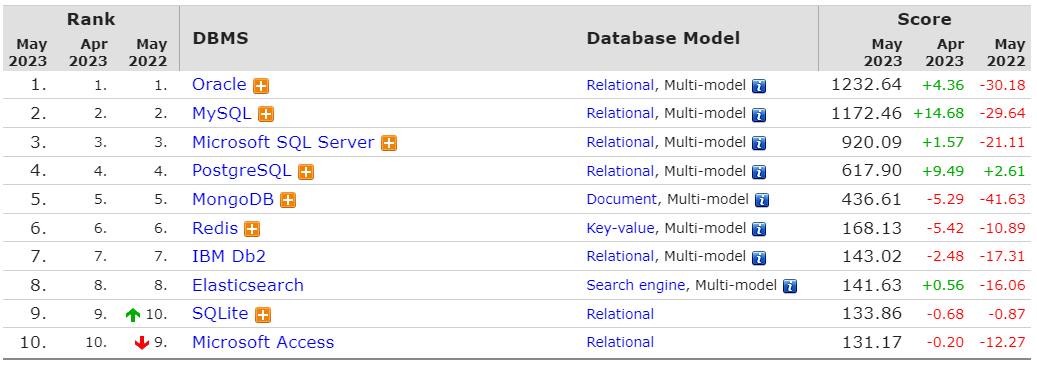
\includegraphics[width=10cm]{./assets/figures/MySQLPopularity.png}
        \caption{Popularité des différents SGBD dans le monde \label{MySQLPopularity.png}}
    \end{figure}
\end{center}
On voit également sur ce classement que les SGBD les plus populaires ont des scores assez similaire et ont tous deux de la marge sur leur concurent qui occupe la troisième place. Oracle étant un SGBDR légèrement plus populaire que MySQL, il aurait pu être intéressant de choisir ce SGBD.

\begin{center}
    \begin{figure}[H]%TODO : Changer la taille de cette image
        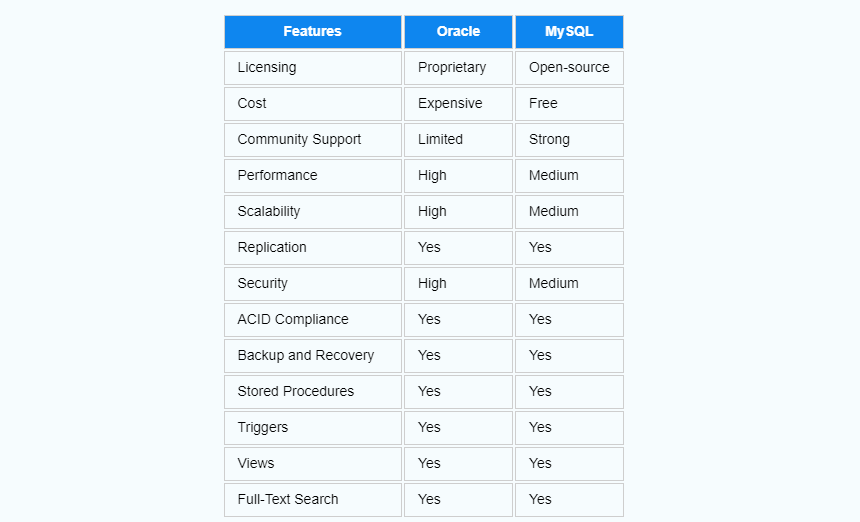
\includegraphics[width=\textwidth]{./assets/figures/OracleVsMySql.png}
        \caption{Comparaison entre Oracle et MySql \label{OracleVsMySql.png}}
    \end{figure}
\end{center}
Cependant comme montré dans l'article du site \href{https://www.integrate.io/blog/oracle-vs-mysql/#:~:text=Oracle%20supports%20distributed%20databases%20while,Oracle%20requires%20a%20licensing%20fee.}{Integrate.io} les avantages sont minimes (des performances un peu meilleures et un sécuritée accrue). La license Oracle étant cependant très onéreuse, Oracle ne fait pas un bon candidat dans le cadre de ce travail de Bachelor.

C'est pourquoi j'ai décidé de rester sur la version 8.0 de MySQL. De plus, grace au framework Laravel il est extrêment simple de changer de SGBD. Il suffit de modifier le fichier de configuration.

\subsection{Laravel}
Laravel est un framework web open-source, écrit en PHP, offrant une structure solide et élégante pour la création d'application et de site web. Le but principal de ce framework est de simplifier la création et le développement d'application grâce à des fonctionnalités intégrées au framework. On y retrouve la gestion de routes, les sessions, l'authentification des utilisateurs ainsi que la gest de la base de données.
Laravel fourni un ORM (Object Relational Mapping), appelé Eloquent permettant de gérer toutes les intercations avec la base de données. Il permet également de choisir avec quel type de SGBD nous souhaitons travailler et de changer ce dernier très rapidement grâce à des fichiers de configuration.
Il propose un pattern architechturale très utilisé, le Modèle-Vue-Controller.
\begin{center}
    \begin{figure}[H]%TODO : Changer la taille de cette image
        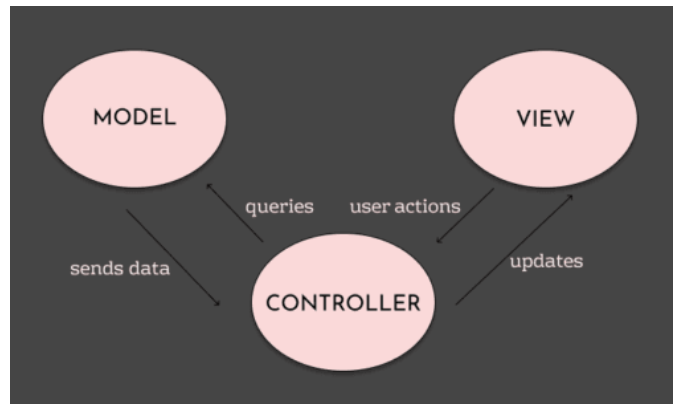
\includegraphics[width=\textwidth]{./assets/figures/MVCExplanation.png}
        \caption{Représentation du MVC \label{MVCExplanation.png}}
    \end{figure}
\end{center}

Sur cette capture, tirée du site \href{https://pusher.com/blog/laravel-mvc-use/#what-is-mvc}{Pusher}, on peut voir les trois parties de ce système et comment elles interagissent.
\begin{itemize}
    \item Le Modèle est la partie responsable de la gestion des données ainsi que de la logique métier. C'est la seule partie du pattern qui interagit avec la base de données. Il représente les structures de données, et fourni au Controller des méthodes pour manipuler les données.
    \item La vue est la partie qui gère de l'interface utilisateur. Elle affiche les données et permet également de récupérer les informations saisies par l'utilisateur notamment au travers de formulaires.
    \item Le Controller est la partie qui lie le Modèle et la Vue. Il réagit aux inputs de l'utilisateur qui sont transmis par la Vue et va interroger, si nécessaire, le Modèle afin d'y metter à jours ou récupérer des données. C'est également lui qui détermine quelle est la Vue à afficher à l'utilisateur. C'est le responsable de la logique de l'application.
\end{itemize}
Le MVC permet donc d'avoir une séparation distincte entre les différentes parties de notre application.

Un autre point fort de Laravel est sa gestion des middleware. Un Middleware est une sorte de filtre qui intervient lorsque les requêtes HTTP arrivent dans notre application. Cela permet notamment d'imposer qu'un utilisateur soit authentifié avant d'accéder à certaines routes ou URL. Ils offre donc un contrôle accru et centralisent la logique de certaines fonctionnalités.

Laravel est donc l'un des framework les plus populaires, simple à prendre en main avec une documentation complète et mise à jour. Il est donc le candidat idéal pour ce projet. De plus, un changement de framework imposerait une charge de travail supplémentaire bien trop conséquente.
Je vais donc utiliser la version 10 de Laravel.

\subsection{Récapitulatif des technologies}
Dans la tableau ci-dessous, vous pouvez trouver la liste de toutes les technologies qui sont utilisée dans le cadre de ce projet ainsi que leur version.